\documentclass{beamer}
\usepackage[utf8]{inputenc}
\usepackage[english]{babel}
\usepackage{amsfonts}
\usepackage{amsmath}
\usepackage{amssymb}
\usepackage{tikz}
\usepackage{float}
\usepackage{pgfplots}
\usetikzlibrary{arrows.meta}
\usetikzlibrary{decorations.markings}
\usepackage{graphicx}

\newcommand{\con}[1]{\mathbb{#1}}
\newcommand{\R}{\con{R}}
\newcommand{\C}{\con{C}}
\newcommand{\Z}{\con{Z}}
\newcommand{\e}{\varepsilon}
\newcommand{\de}{\delta}
\newcommand{\quocient}[2]{{\raisebox{.1em}{$#1$}\left/\raisebox{-.1em}{$#2$}\right.}}

\usetheme{Hannover}

%gets rid of bottom navigation symbols
\setbeamertemplate{navigation symbols}{}

\title{Morse theory and Floer homology}

\author{Joaquim Brugués Mora \\ \ \\ {\it advisors } \\ Eva Miranda Galceran \\ Cédric Oms}

\institute{Facultat de Matemàtiques i Estadística\\ UPC}

\date{\today}

\makeatletter
	\setbeamertemplate{sidebar \beamer@sidebarside}%{sidebar theme}
	{
		\beamer@tempdim=\beamer@sidebarwidth%
		\advance\beamer@tempdim by -6pt%
		\insertverticalnavigation{\beamer@sidebarwidth}%
		\vfill
		\ifx\beamer@sidebarside\beamer@lefttext%
		\else%
			\usebeamercolor{normal text}%
			\llap{\usebeamertemplate***{navigation symbols}\hskip0.1cm}%
			\vskip2pt%
		\fi%
	}%
\makeatother

\begin{document}

\begin{frame}
	\titlepage
\end{frame}

\begin{frame}{Contents}
	\tableofcontents
\end{frame}

\section{Introduction}
\begin{frame}{Example (I)}
	
	Torus embedded in $\R^3$:

	\begin{figure}[h]
		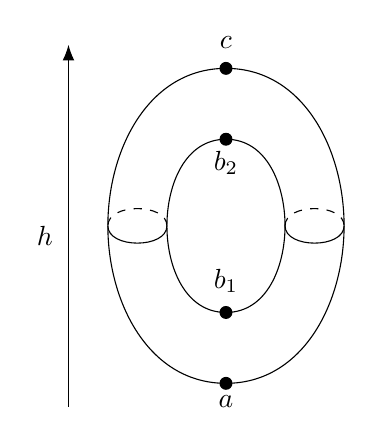
\begin{tikzpicture}
	%Draw the torus
	\draw [] (0,2) to [out=0,in=90] (1.5,0) to [out=270,in=0] (0,-2) to [out=180,in=270] (-1.5,0) to [out=90,in=180] (0,2);
	\draw [] (0.75,0) to [out=270,in=0] (0,-1.1) to [out=180,in=270] (-0.75,0) to [out=90,in=180] (0,1.1) to [out=0,in=90] (0.75,0);
	\draw [] (-1.5,0) to [out=270,in=270] (-0.75,0);
	\draw [dashed] (-0.75,0) to [out=90,in=90] (-1.5,0);
	\draw [] (1.5,0) to [out=270,in=270] (0.75,0);
	\draw [dashed] (0.75,0) to [out=90,in=90] (1.5,0);

	%Critical point c
	\draw [fill] (0,2) circle [radius=0.75mm]
	node [label={[above]$c$}] {};
	%Critical point b_2
	\draw [fill] (0,1.1) circle [radius=0.75mm]
	node [label={[below,yshift=-1.5mm]$b_2$}] {};
	%Critical point b_1
	\draw [fill] (0,-1.1) circle [radius=0.75mm]
	node [label={[above]$b_1$}] {};
	%Critical point a
	\draw [fill] (0,-2) circle [radius=0.75mm]
	node [label={[below,yshift=-1.5mm]$a$}] {};

	%Function h
	\draw [-{Latex[length=2mm]}] (-2,-2.3) to (-2,2.3);
	\draw (-2.3,-0.5) node [label={$h$}]{};
\end{tikzpicture}

		\caption{Critical points in the torus}
		\label{figure:torus1}
	\end{figure}
\end{frame}

\begin{frame}{Example (II)}
	Region under the hypersurface $h(x) = K$:

	\begin{figure}[h]
		\scalebox{.6}{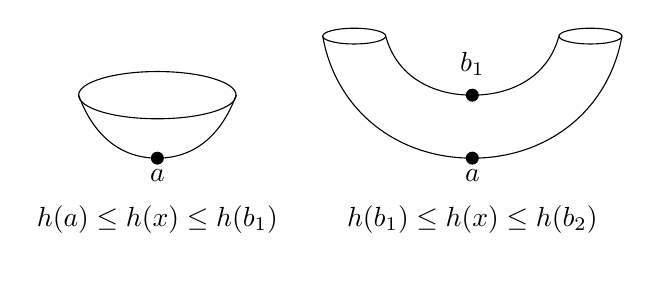
\begin{tikzpicture}
	%Figure at the left
	\draw (-2,0) ellipse (1cm and 3mm);
	%Connection
	\draw (-3,0) to [out=290,in=180] (-2,-0.8) to [out=0,in=250] (-1,0);
	%Critical point a
	\draw [fill] (-2,-0.8) circle [radius=0.75mm]
	node [label={[below,yshift=-1.5mm]$a$}] {};
	%Label of the region
	\draw (-2,-2) node [label={$h(a) \leq h(x) \leq h(b_1)$}]{};

	%Figure at the right
	%End circles of the cilinder
	\draw (0.5,0.75) ellipse (4mm and 1mm);
	\draw (3.5,0.75) ellipse (4mm and 1mm);
	\draw (0.9,0.75) to [out=285,in=180] (2,0) to [out=0,in=255] (3.1,0.75);
	\draw (0.1,0.75) to [out=280,in=180] (2,-0.8) to [out=0,in=260] (3.9,0.75);
	%Critical point b_1
	\draw [fill] (2,0) circle [radius=0.75mm]
	node [label={[above]$b_1$}] {};
	%Critical point a
	\draw [fill] (2,-0.8) circle [radius=0.75mm]
	node [label={[below,yshift=-1.5mm]$a$}] {};
	%Label of the region
	\draw (2,-2) node [label={$h(b_1) \leq h(x) \leq h(b_2)$}]{};
\end{tikzpicture}
}
		\scalebox{.6}{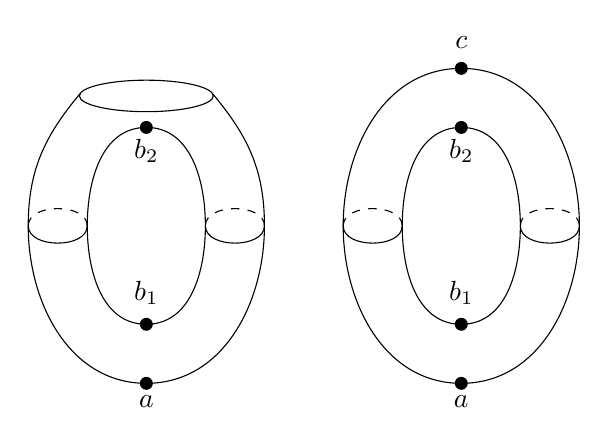
\begin{tikzpicture}
	%Figure at the left
	\draw [] (-1.16,1.68) to [out=310,in=90] (-0.5,0) to [out=270,in=0] (-2,-2) to [out=180,in=270] (-3.5,0) to [out=90,in=230] (-2.84,1.68);
	\draw [] (-1.25,0) to [out=270,in=0] (-2,-1.25) to [out=180,in=270] (-2.75,0) to [out=90,in=180] (-2,1.25) to [out=0,in=90] (-1.25,0);
	\draw [] (-0.5,0) to [out=270,in=270] (-1.25,0);
	\draw [dashed] (-0.5,0) to [out=90,in=90] (-1.25,0);
	\draw [] (-2.75,0) to [out=270,in=270] (-3.5,0);
	\draw [dashed] (-2.75,0) to [out=90,in=90] (-3.5,0);

	%Section at the top
	\draw (-2,1.65) ellipse (8.5mm and 2mm);

	%Critical point b_2
	\draw [fill] (-2,1.25) circle [radius=0.75mm]
	node [label={[below,yshift=-1.5mm]$b_2$}] {};
	%Critical point b_1
	\draw [fill] (-2,-1.25) circle [radius=0.75mm]
	node [label={[above]$b_1$}] {};
	%Critical point a
	\draw [fill] (-2,-2) circle [radius=0.75mm]
	node [label={[below,yshift=-1.5mm]$a$}] {};

	%Figure at the right (Torus)
	\draw [] (2,2) to [out=0,in=90] (3.5,0) to [out=270,in=0] (2,-2) to [out=180,in=270] (0.5,0) to [out=90,in=180] (2,2);
	\draw [] (2.75,0) to [out=270,in=0] (2,-1.25) to [out=180,in=270] (1.25,0) to [out=90,in=180] (2,1.25) to [out=0,in=90] (2.75,0);
	\draw [] (0.5,0) to [out=270,in=270] (1.25,0);
	\draw [dashed] (0.5,0) to [out=90,in=90] (1.25,0);
	\draw [] (2.75,0) to [out=270,in=270] (3.5,0);
	\draw [dashed] (2.75,0) to [out=90,in=90] (3.5,0);

	%Critical point c
	\draw [fill] (2,2) circle [radius=0.75mm]
	node [label={[above]$c$}] {};
	%Critical point b_2
	\draw [fill] (2,1.25) circle [radius=0.75mm]
	node [label={[below,yshift=-1.5mm]$b_2$}] {};
	%Critical point b_1
	\draw [fill] (2,-1.25) circle [radius=0.75mm]
	node [label={[above]$b_1$}] {};
	%Critical point a
	\draw [fill] (2,-2) circle [radius=0.75mm]
	node [label={[below,yshift=-1.5mm]$a$}] {};
\end{tikzpicture}
}
		\caption{Formation of the torus}
		\label{figure:torus2}
	\end{figure}
\end{frame}

\begin{frame}{Reeb theorem}
	\begin{block}{Idea}
		The critical points of the function give information about the topology of the manifold.

		%Conversely, the topology of a manifold restricts the number of critical points.
	\end{block}

	\begin{figure}[h]
		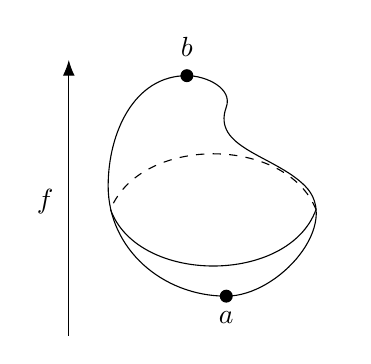
\begin{tikzpicture}
	%Potato-like figure
	\draw [] (0,0) to [out=180,in=270] (-1.5,1.4) to [out=90,in=180] (-0.5,2.8) to [out=0,in=70] (0,2.4) to [out=250,in=135] (1,1.4) to [out=315,in=0] (0,0);
	\draw [] (-1.47,1.1) to [out=290,in=250] (1.14,1.1);
	\draw [dashed] (1.14,1.1) to [out=112,in=68] (-1.47,1.1);

	%Critical point a
	\draw [fill] (0,0) circle [radius=0.75mm]
	node [label={[below,yshift=-2mm]$a$}] {};
	%Critical point b
	\draw [fill] (-0.5,2.8) circle [radius=0.75mm]
	node [label={[above]$b$}] {};

	%Function f
	\draw [-{Latex[length=2mm]}] (-2,-0.5) to (-2,3);
	\draw (-2.3,0.8) node [label={$f$}]{};
\end{tikzpicture}

		\label{figure:reebtheorem}
	\end{figure}

	\begin{theorem}
		{\bf (Reeb):} If $M$ is a compact, connected manifold without boundary and $f : M \rightarrow \R$ is smooth and has only 2 critical points, then $M \cong \con{S}^n$.
	\end{theorem}
\end{frame}

\section{Morse homology}

\begin{frame}{Morse complex}
	\begin{block}{Definition}
		A {\bf complex chain} is a sequence of groups and morphisms
		\[\cdots \rightarrow C_{k+1} \xrightarrow[]{\partial_{k+1}} C_k \xrightarrow[]{\partial_k} C_{k-1} \rightarrow \cdots\]
		with $\partial_k \circ \partial_{k+1} = 0$.

		The {\bf homology groups} of a complex are
		\[H_k = \quocient{\mathrm{Ker} \partial_k}{\mathrm{Im} \partial_{k+1}}\]
	\end{block}

	There are several ways to define a homology over a manifold, capturing topological information about it.
\end{frame}

\begin{frame}{Scheme of construction}
	In both Morse and Floer homology, we take the same steps to define the homology:
	\begin{itemize}
		\item Define object of study and its regularity conditions.
		\item Define an index to classify the objects.
		\item Provide a way to connect objects of consecutive indices. From this, construct the differential $\partial$.
	\end{itemize}
\end{frame}

\begin{frame}{Morse functions}
	\begin{block}{Definition}
		A critical point $p$ of a function $f : M \rightarrow \R$ is {\bf non-degenerate} if its Hessian at $p$ is non-degenerate, this means, does not have $0$ as an eigenvalue.

		A function $f$ is a {\bf Morse function} if all its critical points are non-degenerate.

		The {\bf index} of a non-degenerate critical point $p$, $\mathrm{Ind}(p)$ is the number of negative eigenvalues of the Hessian at $p$.
	\end{block}

	\begin{block}{Morse complex groups}
		The $k$-th group of the Morse complex is
		\[CM_k(M,f) = \bigoplus_{\substack{c \in \mathrm{Crit}(f) \\ \mathrm{Ind}(c) = k}} \con{Z}_2 c\]
	\end{block}
\end{frame}

\begin{frame}{Morse Lemma}
	\begin{theorem}
		If $f : M \rightarrow \R$ is a Morse function, for any critical point $p$ there is a chart $U$ centered at $p$ such that the local expression of $f$ is
		\[\left. f\right|_U(x_1,...,x_n) = f(p) - x_1^2 - \cdots - x_k^2 + x_{k+1}^2 + \cdots + x_n^2,\]
		where $k = \mathrm{Ind}(p)$.
	\end{theorem}

	\begin{figure}
		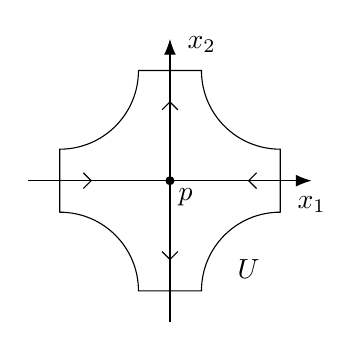
\begin{tikzpicture}
	%Axis
	\draw [-{Latex[length=2mm]}] (-1.8,0) to (1.8,0);
	\draw [-{Latex[length=2mm]}] (0,-1.8) to (0,1.8);
	\draw (1.8,-0.2) node [label={[below]$x_1$}]{};
	\draw (0.1,1.6) node [label={[right]$x_2$}]{};
	%Point p
	\draw [fill] (0,0) circle [radius=0.5mm]
	node [label={[below,xshift=2mm,yshift=-1mm]$p$}] {};
	%Chart U
	\draw (-0.4,1.4) to (0.4,1.4) to [out=270,in=180] (1.4,0.4) to (1.4,-0.4) to [out=180,in=90] (0.4,-1.4) to (-0.4,-1.4) to [out=90,in=0] (-1.4,-0.4) to (-1.4,-0.4) to (-1.4,0.4) to [out=0,in=270] (-0.4,1.4);
	\draw (1,-1) node [label={[below]$U$}]{};
	%Arrows
	\draw (1.1,0.1) to (1,0) to (1.1,-0.1);
	\draw (-1.1,0.1) to (-1,0) to (-1.1,-0.1);
	\draw (-0.1,0.9) to (0,1) to (0.1,0.9);
	\draw (-0.1,-0.9) to (0,-1) to (0.1,-0.9);
\end{tikzpicture}
		\label{figure:morse_chart}
		\caption{A Morse chart for the function $f$}
	\end{figure}
\end{frame}

\begin{frame}{Differential}
	To define the differential $\partial$ on the Morse complex, we connect the critical points of $f$ using the flow of the negative gradient:
	\[\dot{x} = - \mathrm{grad}_x (f)\]

	Then, if $n(a,b)$ is the number of trajectories connecting $a$ and $b$ (modulo 2),
	\[\partial_k(a) = \sum_{\substack{b \in \mathrm{Crit}(f) \\ \mathrm{Ind}(b) = k-1}} n(a,b) b\]

	\begin{block}{Problem}
		To guarantee that $n(a,b)$ is well defined, we need to assume that $\mathrm{grad}(f)$ satisfies the {\bf Smale condition}:
		\[W^S(a) \pitchfork W^U(b)\]
		A slight perturbation of $\mathrm{grad}(f)$ satisfies this condition.
	\end{block}
\end{frame}

\begin{frame}{Results}
	Even though the complex $CM_{\bullet}(M,f)$ depends on $f$, the homology $HM_{\bullet}(M)$ is a {\bf topological invariant}.

	\begin{theorem}
		{\bf Morse inequalities:} Let $f : M \rightarrow \R$ a Morse function, $c_k$ the number of critical points of index $k$, and $\beta_k$ the $k$-th Betti number of $M$. Then,
		\[c_k \geq \beta_k\]
		In particular,
		\[\# \mathrm{Crit}(f) \geq \sum_{k=0}^n \beta_k\]
	\end{theorem}
\end{frame}

\section{Floer homology}

\begin{frame}{Symplectic manifolds}
	\begin{block}{Definition}
		A {\bf symplectic structure} on a $2n$-dimensional manifold $M$ is a 2-form $\omega$ that is
		\begin{itemize}
			\item Closed: $d\omega = 0$.
			\item Non-degenerate $\omega(X,\cdot) \neq 0 \ \forall X$.
		\end{itemize}
	\end{block}

	\begin{block}{Motivation}
		It provides the setting to define Hamiltonian systems in manifolds. If $H : M \rightarrow \R$ is an energy function, then the vector field $X_H$ with
		\[\omega(X_H,Y) = -dH(Y) \ \forall Y\]
		generalizes Hamilton's equations for $H$.
	\end{block}
\end{frame}

\begin{frame}{Arnold conjecture}
	\begin{theorem}
		Consider $H_t : \R \times M \rightarrow \R$ a time-dependent Hamiltonian. Then, if $N$ is the number of periodic orbits of $X_{H_t}$,
		\[N \geq \sum_{k=0}^{2n} \beta_k\]
	\end{theorem}

	\begin{block}{Remark}
		In the case of an autonomous Hamiltonian $H$, this is a consequence of the Morse inequalities.
	\end{block}
\end{frame}

\begin{frame}{Assumptions}
	\begin{block}{Scheme}
		We will construct a complex as in the case of Morse theory, but this time it will be generated by the periodic orbits of $X_{H_t}$.

		However, we need to make some assumptions.
	\end{block}
	\begin{itemize}
		\item {\bf Asphericallity:} We assume that any sphere contained in $M$ is contractible to a point (even though weaker conditions can be taken).
		\item {\bf Contractible loops:} We only consider the loops $x : \con{S}^1 \rightarrow M$ that are contractible to a point.
	\end{itemize}
\end{frame}

\begin{frame}{The Floer complex}
	\begin{itemize}
		\item The complex is generated by the 1-periodic and contractible solutions of
		\[\dot{x} = X_{H_t}(x)\]
		The non-degeneracy condition, in this case, is that $\mathrm{det}(d_{x(0)}\varphi_{X_t}^1 - \mathrm{Id}) \neq 0$.
		\item We classify the periodic orbits using the {\bf Conley-Zehnder index}
		\[\mu_{CZ} : SP(M) \longrightarrow \con{Z}\]
		\item The connection between periodic solutions comes from finite energy solutions of the {\bf Floer equation}
		\[\frac{\partial u}{\partial s} + J \frac{\partial u}{\partial t} + \mathrm{grad}_uH_t = 0\]
	\end{itemize}
\end{frame}

\begin{frame}{The Floer equation (I)}
	The {\bf action functional} is
	\[\mathcal{A}_H(x) = \int_0^1 H_t(x(t)) dt - \int_{\con{D}^2} u^{\ast} \omega\]

	\begin{block}{Proposition}
		A loop $x$ is a critical point of $\mathcal{A}_H$ if and only if $\dot{x} = X_{H_t}(x)$.
	\end{block}
\end{frame}

\begin{frame}{The Floer equation (II)}
	\begin{block}{Definition}
		An {\bf almost complex structure} $J$ on $M$ is a section of $TM\otimes TM^{\ast}$ such that
		\[J^2 = - \mathrm{Id}\]
		An almost complex structure and a symplectic structure induce a Riemannian metric $g$ on $M$.
	\end{block}

	Then, the {\bf gradient of} $\mathcal{A}_H$ is
	\[\mathrm{grad}_x\mathcal{A}_H = J \dot{x} + \mathrm{grad}_{x(t)}H_t\]
	The negative gradient flow trajectories of $\mathrm{grad}_x\mathcal{A}_H$ are $u : \R \times \con{S}^1 \rightarrow M$ with
	\[\frac{\partial u}{\partial s} + J \frac{\partial u}{\partial t} + \mathrm{grad}_uH_t = 0\]
\end{frame}

\begin{frame}{The Floer equation (III)}
	\begin{itemize}
		\item The stationary solutions are the periodic solutions of the Hamilton equations
		\[\dot{x} = X_{H_t}(x)\]
		\item The solutions with $\frac{\partial u}{\partial t} = 0$ are negative gradient flow lines
		\[\frac{\partial u}{\partial s} = - \mathrm{grad}_uH_t\]
		They connect critical points (if $H$ does not depend on time).
		\item If $\mathrm{grad}_uH_t = 0$, then the Floer equation is the Cauchy-Riemann equation
		\[\frac{\partial u}{\partial s} + J \frac{\partial u}{\partial t} = 0\]
	\end{itemize}
\end{frame}

\begin{frame}{The Floer equation (IV)}
	To guarantee that the solutions connect critical points of $\mathcal{A}_H$ we need to add the condition that
	\[E(u) < + \infty\]

	\begin{block}{Definition}
		The {\bf energy} of a solution of the Floer equation is
		\[E(u) = \int_{\R \times \con{S}^1} \left| \frac{\partial u}{\partial s} \right|^2 dsdt = \int_{\R \times \con{S}^1} \left| \frac{\partial u}{\partial t} - X_{H_t} \right|^2 dsdt\]
	\end{block}

	\begin{block}{Remark}
		We have that $E(u) = 0$ if and only if $u(s,t) = x(t)$ and it is a periodic solution.
	\end{block}
\end{frame}

\begin{frame}{Results}
	\begin{theorem}
		The Floer homology $HF_{\bullet}(M)$ is a {\bf topological invariant}: it does not depend on $H_t$ or in $J$.
	\end{theorem}

	\begin{theorem}
		The Floer homology of a manifold is isomorphic to the Morse homology:
		\[HF_{\bullet}(M) \cong HM_{\bullet}(M)\]
	\end{theorem}
\end{frame}

\section{Conclusions}

\begin{frame}{Conclusions}
	\begin{itemize}
		\item The Arnold conjecture is proved using the Floer homology in the case of aspherical manifolds.
		\item Moreover, this technique paves the way for the general proof.
		\item The scheme used to define the Morse complex is the one used to define the Floer complex.
	\end{itemize}
\end{frame}

\begin{frame}
	\begin{center}
		\huge Thank you for your attention!
	\end{center}
\end{frame}

\end{document}
